This report presents a length-based assessment of the multi-species deep slope fisheries targeting mostly snappers, groupers and emperors, at depths ranging from 50 to 500 meters, in fisheries management area (WPP) 718 in the Arafura Sea in Eastern Indonesia. Drop line and long line vessels fish in this area together with a number of gear types including bottom trawls that go under the name of "fish net". Bottom long line vessels fish on the shelf area as well as on the top of the slopes that drop to deeper waters. Drop liners fish those slopes also to greater depths into the Banda Sea and the Timor Trough. All gear types operate on both sides of the borders of WPP 718 and neighboring areas, where habitats are continuous, often within a single fishing trip.

Various fleets are operating in this region, including long liners and drop liners from Bali (often via Kupang), long liners from Probolinggo, Timika, Dobo, Tual, drop liners from Kema (North Sulawesi) and Ternate and trawlers from Sorong, Timika and other bases. Vessels from most of these fleets contributed data to the current assessment. Some vessels are based and operate entirely within the WPP 718 boundaries others like some of the medium scale drop liners from Kema and Ternate make trips to locations up to 1,000 kilometers away from their home ports. Various staging points and logistical hubs are used by the Arafura Sea fishing fleets, throughout Eastern Indonesia.

The drop line fishery is an active vertical hook and line fishery operating at depths from 50 to 500 meters, whereas long lines are set horizontally along the bottom at depths ranging from 50 to 150 meters. Trawlers work mostly over the shallower parts of the shelf area at depths overlapping mostly with the long line fisheries.

This report analyzes length frequencies of the 50 species of fish that were the most abundant in the combined drop and long line fisheries operating in WPP 718. For a complete overview of the species composition please refer to the ID guide prepared for these fisheries:

\textbf{CLICK: }\href{http://72.14.187.103:8080/ifish/pub/TNC_FishID.pdf}{Link to on-line E-Book Species ID Guide}

For further background on species life history characteristics, and data-poor length based assessment methods, as applied in this report, please refer to the assessment guide that was separately prepared for these fisheries:

\textbf{CLICK: }\href{http://72.14.187.103:8080/ifish/pub/DeepSlopeSpeciesAssessmentTool.pdf}{Link to on-line E-Book Assessment Guide with Biological Information}

Data in this report represent complete catches by small and medium scale vessels from the above described fleets. All fish captured were photographed on measuring boards by fishing crew participating in our Crew Operated Data Recording System or CODRS. Images were analyzed by project staff to generate the species specific length frequency distributions of the catches which served as the input for our length based assessment of this fishery.

\begin{center}
\graphicspath{{/root/R-project/IFishSnapperWPP718/Images/}}
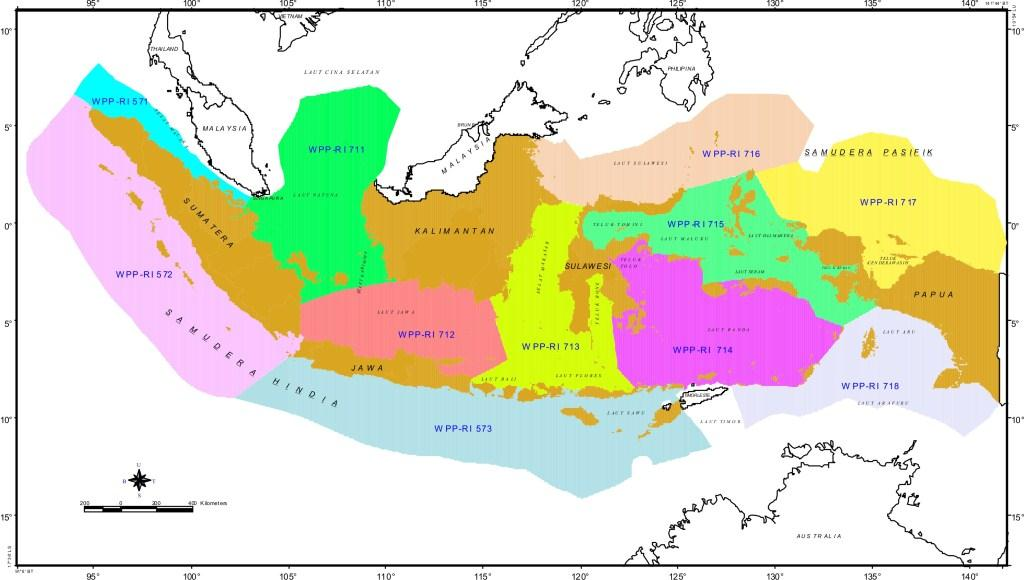
\includegraphics[scale=1.8]{wpp-indonesia.jpg}

Figure 1. Fisheries Management Areas (WPP) in Indonesian marine waters.
\end{center}

\begin{center}
\graphicspath{{/root/R-project/IFishSnapperWPP718/Images/}}
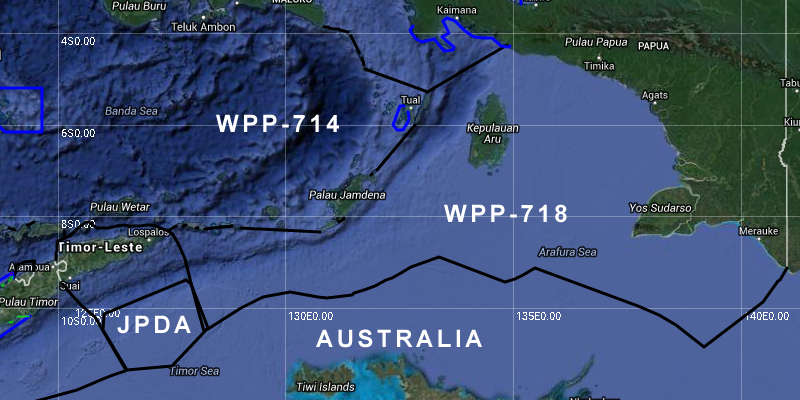
\includegraphics[scale=0.55]{AreaD-Satellite.png}

Figure 2. Bathymetric map of the Arafura Sea, WPP 718, with adjacent marine areas, in Eastern Indonesia. Black lines are WPP boundaries, blue lines are MPA boundaries.
\end{center}